\section{Giới thiệu}
Lưu ý tất cả nội dung trong các mục này đều chỉ mang tính minh họa. \lipsum[4][1-3]
\subsection{Tổng quan về bệnh ung thư}
\lipsum[1]\\
\lipsum[2]
\subsection{Cơ chế gây bệnh ung thư}
\lipsum[3]
\section{Mô hình toán học}
\subsection{Các giả định}
\lipsum[2]
\begin{itemize}
    \item The penguin is a cylinder. \lipsum[9][1-3]

    \item Friction is ignored. \lipsum[3][1-3]

    \item \lipsum[4][1-3]

    \item \lipsum[5][1-3]
\end{itemize}

\subsection{Xây dựng mô hình}

\lipsum[3][1-8]\\
\begin{align}\label{equation_1}
    \begin{split}
        \begin{cases}
            y_t - \Delta y + (y \cdot\nabla)y + \nabla p = f(x,t) \text{ in }Q:=\Omega \times (0;T);\\
            \nabla \cdot y = 0 \text{ in }Q; \,y(0,t)=y_0(t) \text{ on }(0;T); \, y(x,t) = 0 \text{ on }\partial\Omega \times (0;T).
        \end{cases}
    \end{split}
\end{align}

The equation \eqref{equation_1} determined the velocity $y(x,t)$ and the scalar pressure $p(x,t)$ at each point in the domain $\Omega$. \lipsum[4]


\section{Kết quả và mô phỏng}
Use the table and tabular environments for basic tables --- see Tables~\ref{tab1} and \ref{tab2}, for example. Table \ref{tab1} is an sample figure including table footnotes. For more information, please see this help article on \href{https://www.overleaf.com/learn/latex/tables}{tables}. 

\begin{table}[!ht]
\caption{Sample table with footnotes\label{tab1}}
\begin{threeparttable}
\begin{tabular*}{\columnwidth}{@{\extracolsep\fill}llll@{\extracolsep\fill}}
\toprule
column 1 & column 2 & column 3 & column 4\\
\midrule
row 1 & data 1 & data 2 & data 3 \\
row 2 & data 4 & data 5\tnote{1} & data 6 \\
row 3 & data 7 & data 8 & data 9\tnote{2} \\
\bottomrule
\end{tabular*}
\begin{tablenotes}
\item Source: This is an example of table footnote. This is an example of table footnote. This is an example of table footnote. This is an example of table footnote. This is an example of table footnote.
\item[1] Example of a first table footnote.
\item[2] Example of a second table footnote.
\end{tablenotes}
\end{threeparttable}
\end{table}

\lipsum[4]
\begin{table*}[!h]
\caption{Example of a lengthy table which is set to full textwidth.\label{tab2}}
\tabcolsep=0pt
\begin{threeparttable}
\begin{tabular*}{\textwidth}{@{\extracolsep{\fill}}lcccccc@{\extracolsep{\fill}}}
\toprule
& \multicolumn{3}{c}{Element 1\tnote{1}} & \multicolumn{3}{c}{Element 2\tnote{2}} \\
\cmidrule(lr){2-4}\cmidrule(lr){5-7}
Project & Energy & $\sigma_{\mathrm{calc}}$ & $\sigma_{\mathrm{expt}}$ & Energy & $\sigma_{\mathrm{calc}}$ & $\sigma_{\mathrm{expt}}$ \\
\midrule
Element 3 & 990 A & 1168 & $1547\pm12$ & 780 A & 1166 & $1239\pm100$ \\
Element 4 & 500 A & 961 & $922\pm10$ & 900 A & 1268 & $1092\pm40$ \\
\bottomrule
\end{tabular*}
\begin{tablenotes}
\item Note: This is an example of table footnote this is an example of table footnote this is an example of table footnote this is an example of~table footnote this is an example of table footnote.
\item[1] Example of a first table footnote.
\item[2] Example of a second table footnote.
\end{tablenotes}
\end{threeparttable}
\end{table*}

As per display \LaTeX\ standards one has to use eps images for \verb+latex+ compilation and \verb+pdf/jpg/png+ images for
\verb+pdflatex+ compilation. This is one of the major differences between \verb+latex+
and \verb+pdflatex+. The images should be single-page documents. The command for inserting images
for \verb+latex+ and \verb+pdflatex+ can be generalized. The package used to insert images in \verb+latex+ is the
graphicx package. Figures can be inserted via the normal figure environment as shown in the below example:


\begin{figure}[!h]
        \centering
        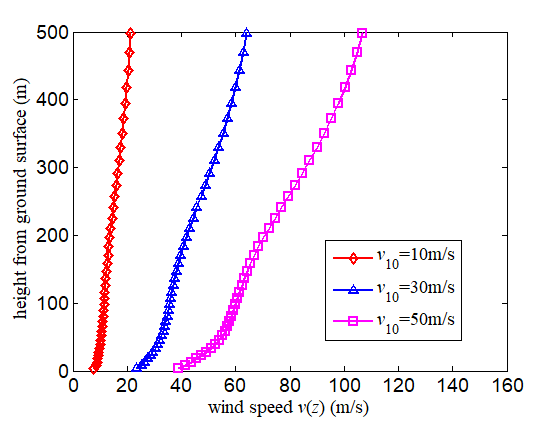
\includegraphics[width=0.5\linewidth]{Image/fig_a.png}
        \caption{Figure example}
\end{figure}

\lipsum[3][1-5]

\section{Kết luận}
\subsection{Ưu điểm của mô hình}
\lipsum[4][1-7]

\begin{enumerate}
    \item \lipsum[4][1-3]

    \item \lipsum[4][1-3]

    \item \lipsum[4][1-3]
\end{enumerate}

\subsection{Nhược điểm của mô hình}
\lipsum[4][1-7]

\begin{enumerate}
    \item \lipsum[4][1-3]

    \item \lipsum[4][1-3]

    \item \lipsum[4][1-3]
\end{enumerate}
\subsection{Hướng phát triển mô hình}
\lipsum[4][1-7]

\begin{enumerate}
    \item \lipsum[4][1-3]

    \item \lipsum[4][1-3]

    \item \lipsum[4][1-3]
\end{enumerate}

\newpage
\thispagestyle{empty}
\begin{thebibliography}{99}
\bibitem{1} D.~E. KNUTH   The \TeX{}book  the American
Mathematical Society and Addison-Wesley
Publishing Company , 1984-1986.
\bibitem{2}Lamport, Leslie,  \LaTeX{}: `` A Document Preparation System '',
Addison-Wesley Publishing Company, 1986.
\bibitem{3}\url{https://www.latexstudio.net/}
\end{thebibliography}
\newpage

\begin{appendices}
    \section{First appendix}

In addition, your report must include a letter to the Chief Financial Officer (CFO) of the Goodgrant Foundation, Mr. Alpha Chiang, that describes the optimal investment strategy, your modeling approach and major results, and a brief discussion of your proposed concept of a return-on-investment (ROI). This letter should be no more than two pages in length.

Dear, Mr. Alpha Chiang

\lipsum[1-2]

\vspace{\parskip}

Sincerely yours,

Your friends
\end{appendices}
